\FloatBarrier
\section{Autonomous Walking via Reinforcement Learning}
\label{sec::43_ar}
Since there is to this date no feasible way of training an agent on autonomous navigation in real time with reinforcement learning, we first decided to implement a benchmarking environment, which is introduced in section \ref{sec::431_bpp}, and then to use the benchmarking environment to test the fusion of nonlinear model predictive control with proximal policy optimization in, which is demonstrated in section \ref{sec::431_fpp}.
\subsection{Benchmarking Proximal Policy Optimization}
\label{sec::431_bpp}
To validate the implementation of proximal policy optimization, we used a little benchmarking environment that is shown in figure \ref{fig::431_ppo_env}. The agent's goal within this setup is to move towards the red dot, while keeping a maximum distance of $10\,\text{a.u.}$ towards it. The environment's state is simply described by a concatenation of the agent's position $\bm{a} = \begin{pmatrix}
a_x & a_y
\end{pmatrix}^T$ with that of the goal $\bm{g} = \begin{pmatrix}
g_x & g_y
\end{pmatrix}^T$. The reward $r_t$, at time step $t$, is designed to encourage motion towards the goal, by taking the difference of the previous and the current goal distance $r_t = ||\bm{a}_{t-1}-\bm{g}_{t-1}||_2 - ||\bm{a}_{t}-\bm{g}_{t}||_2$. Furthermore, a reward of ten was gained for successful completion, while a reward of negative ten was granted for whenever the agent left the maximally allowed distance towards the goal, see for example figure \ref{fig::431_ppo_env} (a).
\begin{figure}[h!]
	\centering
	\subcaptionbox{Agent at epoch 1.}%
	[.45\linewidth]{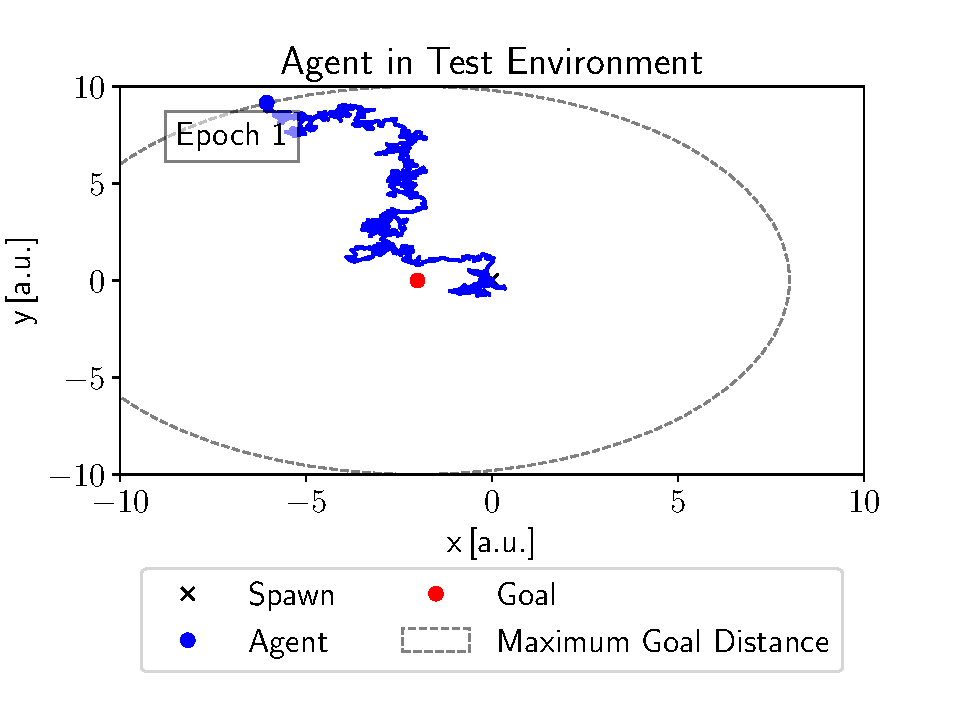
\includegraphics[scale=.45]{chapters/04_experiments/02_autonomous_walking/epoch_1.pdf}}	
	\subcaptionbox{Agent at epoch 30.}%
	[.45\linewidth]{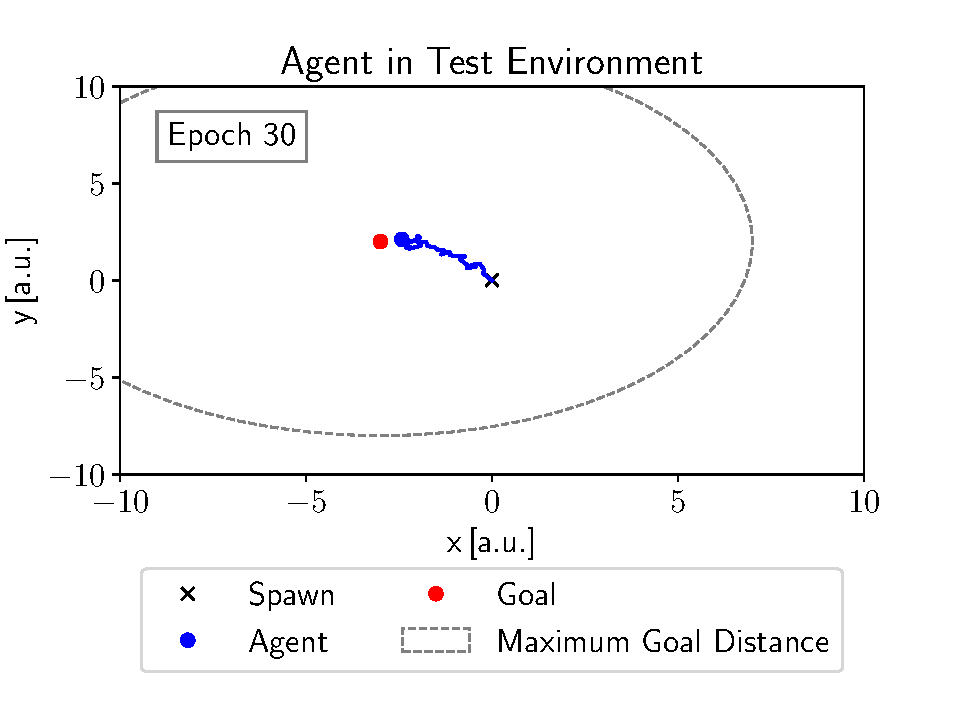
\includegraphics[scale=.45]{chapters/04_experiments/02_autonomous_walking/epoch_30.pdf}}
	\caption{Artificial agent in proximal policy optimization test environment. While the agent acts randomly in epoch 1 (a), the goal is reached with high confidence at epoch 30 (b).}	
	\label{fig::431_ppo_env}
\end{figure} 
In each of the cases, the environment was reset, and the goal got spawned at a random location. For both, the agent and the critic network, we used a fully connected neural network with 2 hidden layers of size 16, and 32, respectively. The output layer provided 2 units, which reflect our agent's degrees of freedom in the environment. For the hidden units, we again relied on rectifying linear units as our activation function, while we used a hyperbolic tangent for the output. We were able to produce the best results with a gradient clipping at $\epsilon=0.2$ (see equation \ref{eq::223_clip}), and the cost function hyper-parameters $c_1 = 0.5$ and $c_2 = 0.1/\overline{r_t}$, where $\overline{r_t}$ denotes the average reward, and which can be found in equation \ref{eq::223_ppo_loss}. 
\begin{figure}[h!]
	\centering
	\subcaptionbox{Reward history.}%
	[.45\linewidth]{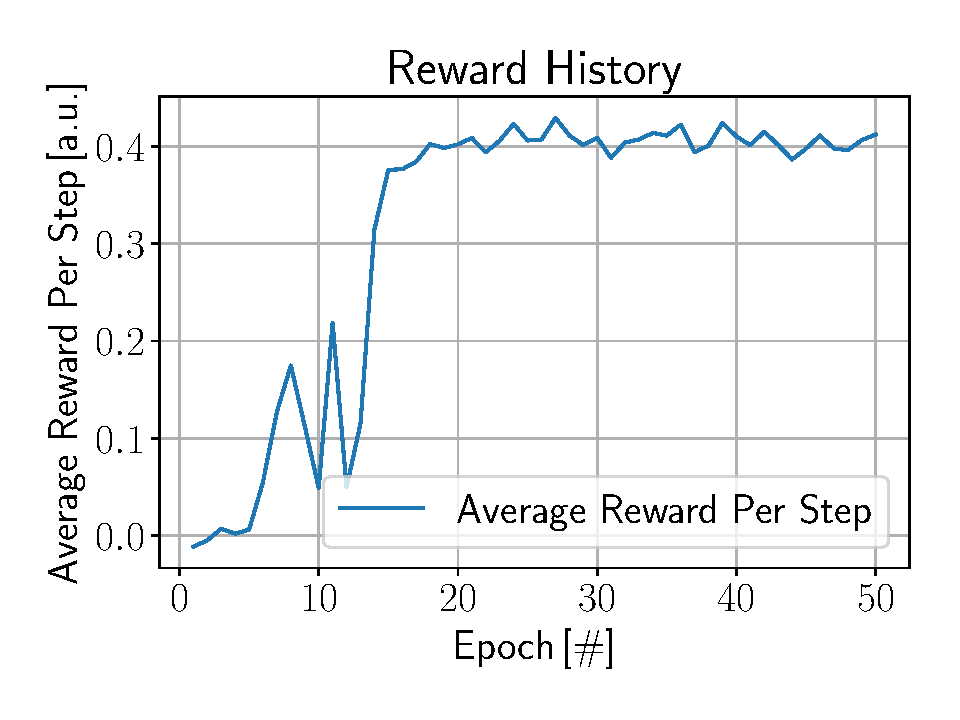
\includegraphics[scale=.35]{chapters/04_experiments/02_autonomous_walking/ppo_reward_history.pdf}}	
	\subcaptionbox{Standard deviation history.}%
	[.45\linewidth]{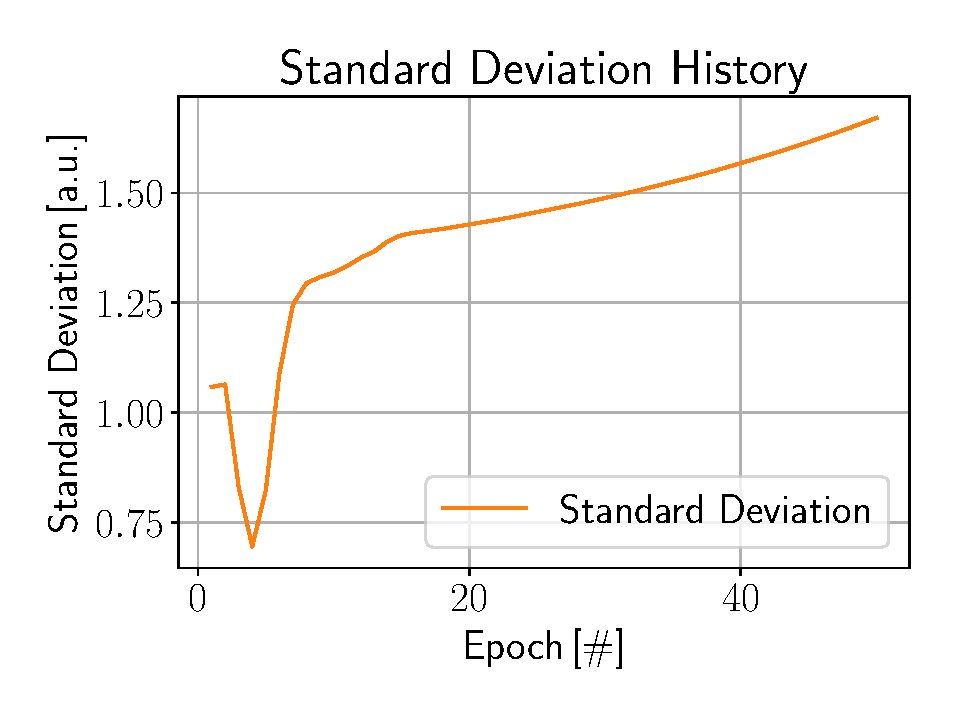
\includegraphics[scale=.35]{chapters/04_experiments/02_autonomous_walking/ppo_std_history.pdf}}
	\caption{Proximal policy optimization in test environment over 50 epochs. The agent learned to maximize the reward after around 20 epochs, by increasing its exploration with a higher standard deviation within the policy $\pi_\theta$ (b).}	
	\label{fig::431_ppo_hist}
\end{figure}
We ran the environment for $10000$ steps per epoch, and updated the networks every $4096$ actions, with a minibatch size of $M=512$ for $8$ proximal policy optimization epochs (see algorithm \ref{alg::225_ac}). The Adam optimizer then led to convergence at a learning rate of $0.01$ after about thirty epochs (see figure \ref{fig::431_ppo_hist}). A main reason for the fast convergence was caused by the chosen entropy hyperparameter $c_2$, which encouraged exploration on low rewards, and damped exploration on high rewards. We computed the entropy $S[\pi_\theta]$ from the differential entropy of our Gaussian policy $\pi_\theta$ via (\href{https://github.com/mhubii/ppo_libtorch/blob/481c1e326dcd6220b2c1c955a0303a410c2cb0dd/Models.h#L82}{\underline{link}})
\begin{align}
S[\pi_\theta] = 0.5 + 0.5\log(2\pi)+\log(\sigma),
\end{align}
where $\sigma$ is the standard deviation. We can then see the standard deviation's influence on the reward, as it starts to increase strongly in figure \ref{fig::431_ppo_hist} (b). After having trained the agent successfully for $50$ epochs, we ran the policy $\pi_\theta$ without noise contribution, but rather took the average $\mu$, as proposed by the actor network. An example of the agent's behavior can be seen in figure \ref{fig::431_ppo_test}, which now appears smooth. 
\begin{figure}[h!]
	\centering
	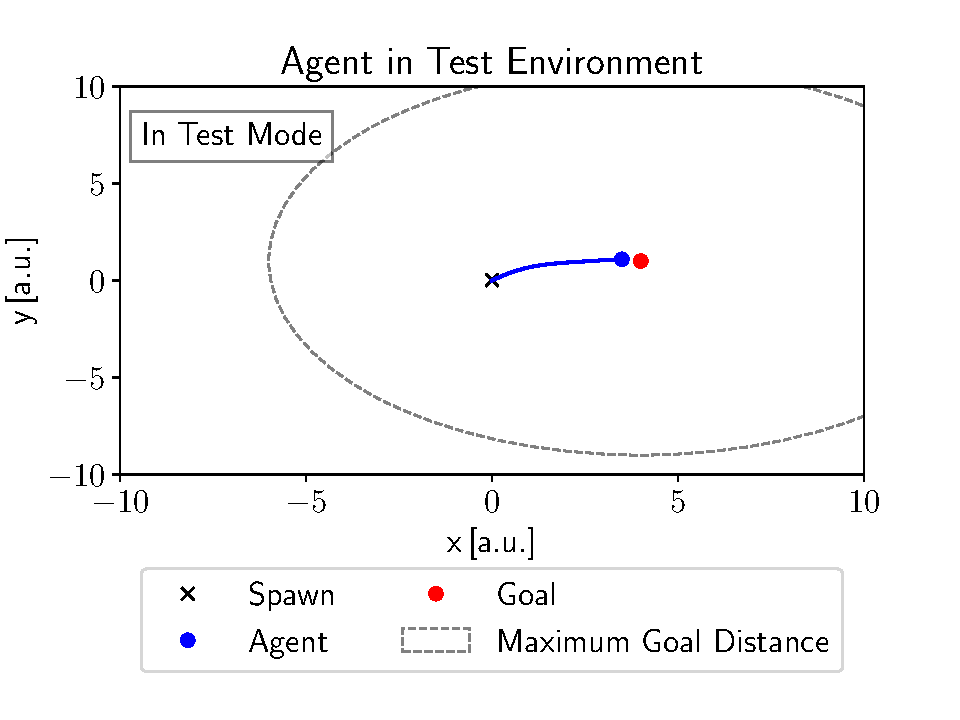
\includegraphics[scale=.45]{chapters/04_experiments/02_autonomous_walking/test_mode.pdf}
	\caption{Proximal policy optimization in test mode that is without noisy policy $\pi_\theta$. The agent almost learned to move the shortest path towards the goal.}	
	\label{fig::431_ppo_test}
\end{figure}
We ran the agent ten times for $10000$ steps without noise contribution, and observed $311\pm3$ wins on average, and no lost game at all, which indicates that the neural network learned to generalize the task well.
\subsection{Fusion of Nonlinear Model Predictive Control with Proximal Policy Optimization}
\label{sec::431_fpp}
For the autonomous navigation, it is then possible to combine proximal policy optimization with nonlinear model predictive control (\href{https://github.com/mhubii/nmpc_pattern_generator/blob/dev/src/train_ppo_nmpc.cpp}{\underline{link}}). Just as in the previous section, a neural network has to solve goal navigation, but this time the agent's trajectories are computed by using the nonlinear model predictive control. The environment's state is simply described by the goal's position $\bm{g}_a=\begin{pmatrix}
g_x & g_y
\end{pmatrix}^T$, as seen from the agent's coordinate frame, which can be expressed by world coordinates via $\bm{g}_a = \bm{R}^{-1}_z(\bm{g}_w-\bm{a}_w)$, where $\bm{R}_z$ is the agent's current rotation, which is given by $\bm{c}_k^\theta[0]$, $\bm{g}_w$ is the goal's position in the world frame, and $\bm{a}_w$ is the agent's position in the world frame. The reward $r_t$ for this task got designed to ensure fast frontal motion towards the goal. It therefore consists of three terms, one of which accounts for motion towards the goal via $r_t^\text{goal} = ||\bm{a}_{t-1}-\bm{g}_{t-1}||_2 - ||\bm{a}_t-\bm{g}_t||_2$, whereas the second term enforces the robot coordinate system's x-axis to point towards the goal via $\bm{r}_t^\text{frontal} = (\bm{g}_{a,t-1}-\bm{g}_{a,t-1})[0]$, and the third term punishes slow paths via $r_t^\text{time}=t$. In total, we found the following weights to work best $r_t=2\cdot10^3r_t^\text{frontal}+6\cdot10^3r_t^\text{goal}-10^{-1}r_t^\text{time}$. An additional reward of $100$ was granted for a successfully finished task. The agent then got trained for 50 epochs, with the Adam optimizer at a learning rate of 0.003. The gradient got clipped at $\epsilon=0.2$, the cost function hyper-parameters were set to $c_1=0.5$, and $c_2=-50$, to ensure a decreasing entropy, as the pattern generator does not allow for arbitrary high commands $v_x$, and $\omega_z$. We ran a single agent $N=1$ for $2000$ preview horizon time-steps, with a mini batch size of $M=200$ for 5 proximal policy optimization epochs (see algorithm \ref{alg::225_ac}). For the network architecture we again chose to go with a fully connected neural network with an input layer of size $2\times64$, two hidden layers at a size of $64\times64$ each, and an output layer of size $64\times2$. The activation functions were set to be hyperbolic tangents. The particular model can be found at the provided \href{https://github.com/mhubii/nmpc_pattern_generator/blob/df058feeb5ba3afd88f2a855e5af148d25c23020/libs/learning/include/learning/models.h#L100}{\underline{link}}. After having fully trained the agent, it was shown that the agent solved the goal navigation task for randomly spawned goals in 100 out of 100 cases. Therefore, we can argue that the agent learned to generalize the task well, and as shown for four exemplary cases in figure \ref{fig::432_nmpc_ppo_env}, the agent also learned to move backwards and turn. 
\begin{figure}[h!]
	\centering
	\subcaptionbox{Goal located at $x=0$, $x=-4$.}%
	[.45\linewidth]{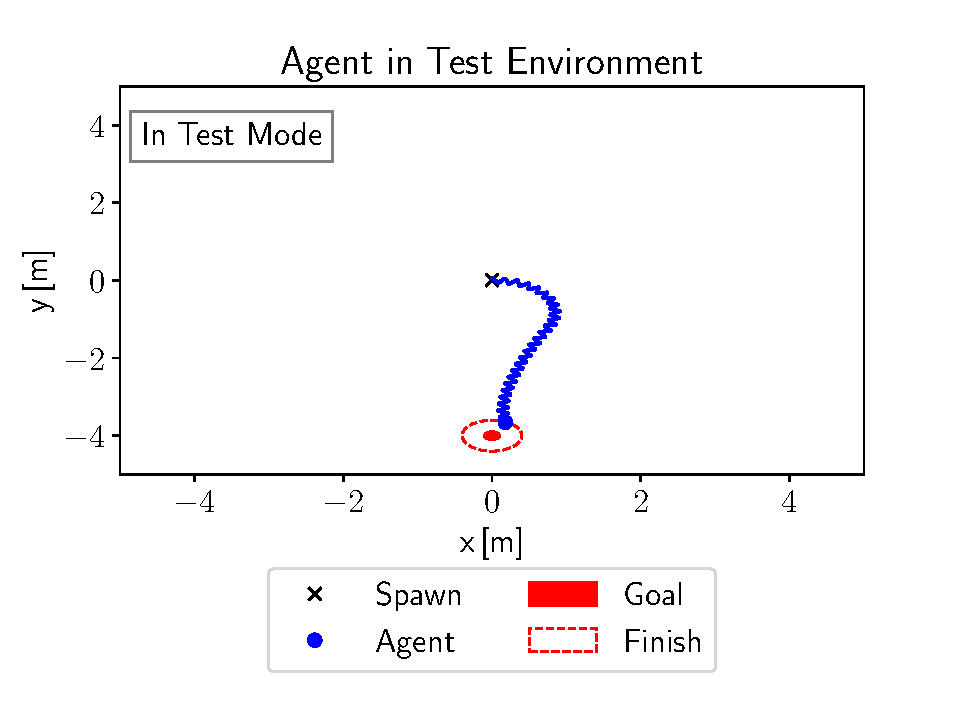
\includegraphics[scale=.45]{chapters/04_experiments/02_autonomous_walking/test_mode_0_m4.pdf}}	
	\subcaptionbox{Goal located at $x=4$, $x=4$.}%
	[.45\linewidth]{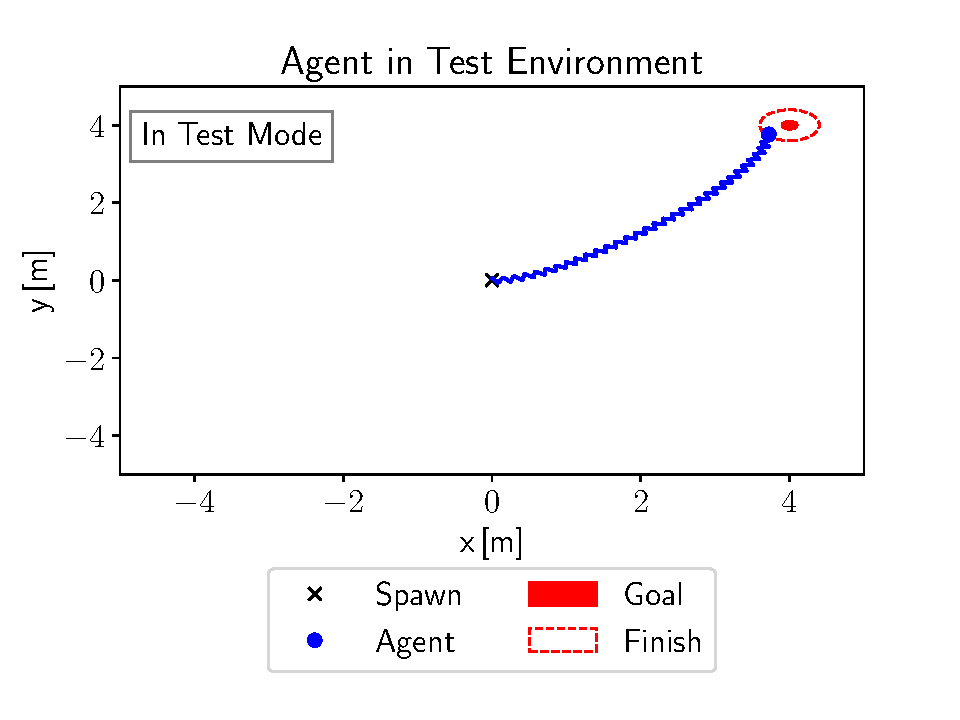
\includegraphics[scale=.45]{chapters/04_experiments/02_autonomous_walking/test_mode_4_4.pdf}}
	\subcaptionbox{Goal located at $x=4$, $x=-4$.}%
	[.45\linewidth]{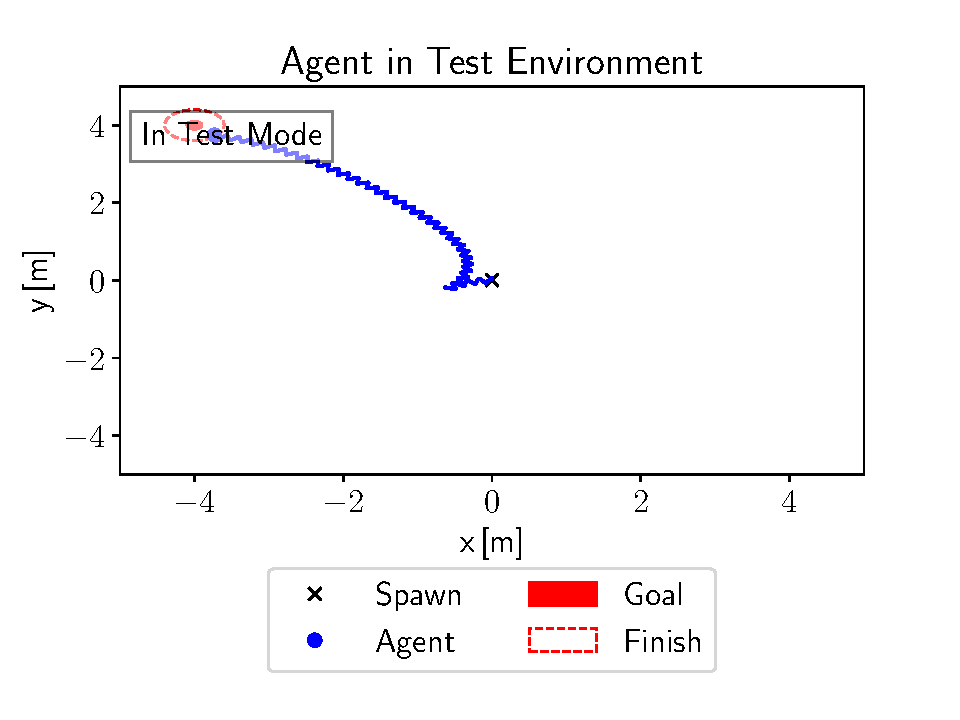
\includegraphics[scale=.45]{chapters/04_experiments/02_autonomous_walking/test_mode_m4_4.pdf}}
	\subcaptionbox{Goal located at $x=-4$, $x=-4$.}%
	[.45\linewidth]{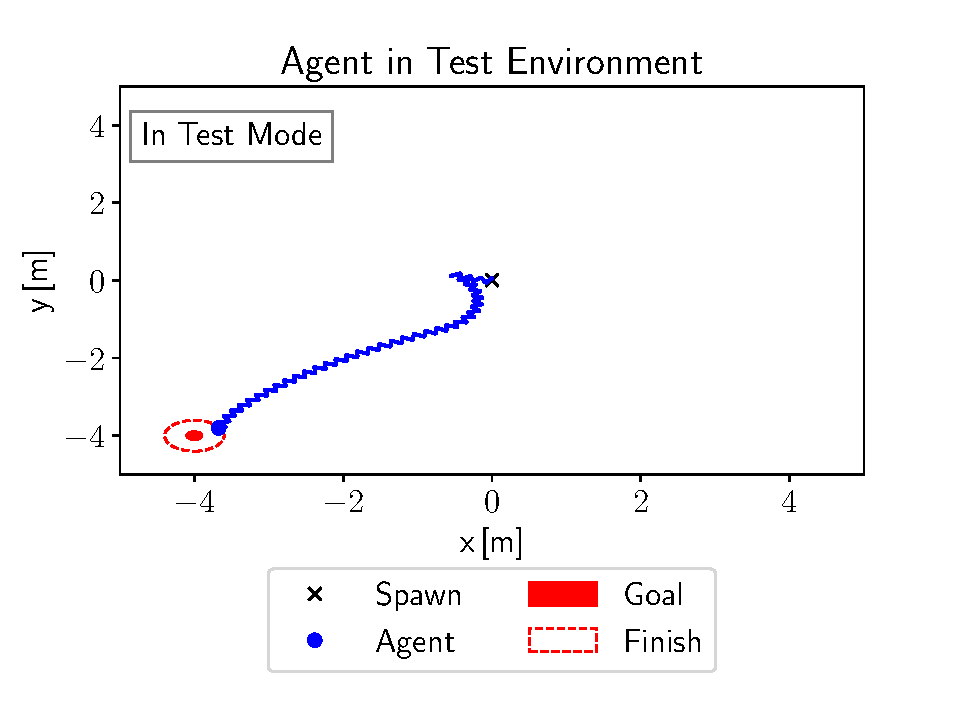
\includegraphics[scale=.45]{chapters/04_experiments/02_autonomous_walking/test_mode_m4_m4.pdf}}
	\caption{Nonlinear model predictive controlled agent in the test environment. The used fully connected neural network successfully learned to steer the NMPC agent in all cases towards the goal, by taking the goal's position as input. Just as in the behavioral cloning setup, the agent was restricted to only send the velocity commands $v_x$, and $\omega_z$ to the NMPC. The trajectories are similar to the ones shown in figure \ref{fig::411_benchmarking_basic}, but only viewed from above. The blue lines, therefore, represent the robot's center of mass trajectories and the robot always faces towards the positive x-direction. Note how the agent learned to turn for the cases (c), and (d).}	
	\label{fig::432_nmpc_ppo_env}
\end{figure} 
